	
% This template from http://www.vel.co.nz, originally from http://www.tedpavlic.com

\documentclass{article}
% Change "article" to "report" to get rid of page number on title page
\usepackage{amsmath,amsfonts,amsthm,amssymb, mathrsfs}
\usepackage{bigints}
\usepackage{setspace}
\usepackage{Tabbing}
\usepackage{fancyhdr}
\usepackage{lastpage}
\usepackage{textcomp}
\usepackage{extramarks}
\usepackage{chngpage}
\usepackage{soul,color}
\usepackage{graphicx,float,wrapfig}
\usepackage{cancel}
\usepackage{indentfirst}
\usepackage{mdframed}

% In case you need to adjust margins:
\topmargin=-0.45in      %
\evensidemargin=0in     %
\oddsidemargin=0in      %
\textwidth=6.5in        %
\textheight=9.0in       %
\headsep=0.25in         %

% Homework Specific Information
\newcommand{\hmwkTitle}{WS16}
\newcommand{\hmwkDueDate}{}
\newcommand{\hmwkClass}{Ay\ 190}
\newcommand{\hmwkAuthorName}{Cutter\ Coryell}

% Setup the header and footer
\pagestyle{fancy}                                                       %
\lhead{\hmwkAuthorName}                                                 %
\chead{\hmwkClass\ : \hmwkTitle}  %
\rhead{\hmwkDueDate}                                                     %
\renewcommand\headrulewidth{0.4pt}                                      %
\renewcommand\footrulewidth{0.4pt}                                      %

% This is used to trace down (pin point) problems
% in latexing a document:
%\tracingall

%%%%%%%%%%%%%%%%%%%%%%%%%%%%%%%%%%%%%%%%%%%%%%%%%%%%%%%%%%%%%
% Some tools
\newcommand{\enterProblemHeader}[1]{\nobreak\extramarks{#1}{#1 continued on next page\ldots}\nobreak%
                                    \nobreak\extramarks{#1 (continued)}{#1 continued on next page\ldots}\nobreak}%
\newcommand{\exitProblemHeader}[1]{\nobreak\extramarks{#1 (continued)}{#1 continued on next page\ldots}\nobreak%
                                   \nobreak\extramarks{#1}{}\nobreak}%

\newlength{\labelLength}
\newcommand{\labelAnswer}[2]
  {\settowidth{\labelLength}{#1}%
   \addtolength{\labelLength}{0.25in}%
   \changetext{}{-\labelLength}{}{}{}%
   \noindent\fbox{\begin{minipage}[c]{\columnwidth}#2\end{minipage}}%
   \marginpar{\fbox{#1}}%

   % We put the blank space above in order to make sure this
   % \marginpar gets correctly placed.
   \changetext{}{+\labelLength}{}{}{}}%

\setcounter{secnumdepth}{0}
\newcommand{\homeworkProblemName}{}%
\newcounter{homeworkProblemCounter}%
\newenvironment{homeworkProblem}[1][Problem \arabic{homeworkProblemCounter}]%
  {\stepcounter{homeworkProblemCounter}%
   \renewcommand{\homeworkProblemName}{#1}%
   \section{\homeworkProblemName}%
   \enterProblemHeader{\homeworkProblemName}}%
  {\exitProblemHeader{\homeworkProblemName}}%

\newcommand{\problemAnswer}[1]
  {\noindent\fbox{\begin{minipage}[c]{\columnwidth}#1\end{minipage}}}%

\newcommand{\problemLAnswer}[1]
  {\labelAnswer{\homeworkProblemName}{#1}}

\newcommand{\homeworkSectionName}{}%
\newlength{\homeworkSectionLabelLength}{}%
\newenvironment{homeworkSection}[1]%
  {% We put this space here to make sure we're not connected to the above.
   % Otherwise the changetext can do funny things to the other margin

   \renewcommand{\homeworkSectionName}{#1}%
   \settowidth{\homeworkSectionLabelLength}{\homeworkSectionName}%
   \addtolength{\homeworkSectionLabelLength}{0.25in}%
   \changetext{}{-\homeworkSectionLabelLength}{}{}{}%
   \subsection{\homeworkSectionName}%
   \enterProblemHeader{\homeworkProblemName\ [\homeworkSectionName]}}%
  {\enterProblemHeader{\homeworkProblemName}%

   % We put the blank space above in order to make sure this margin
   % change doesn't happen too soon (otherwise \sectionAnswer's can
   % get ugly about their \marginpar placement.
   \changetext{}{+\homeworkSectionLabelLength}{}{}{}}%

\newcommand{\sectionAnswer}[1]
  {% We put this space here to make sure we're disconnected from the previous
   % passage

   \noindent\fbox{\begin{minipage}[c]{\columnwidth}#1\end{minipage}}%
   \enterProblemHeader{\homeworkProblemName}\exitProblemHeader{\homeworkProblemName}%
   \marginpar{\fbox{\homeworkSectionName}}%

   % We put the blank space above in order to make sure this
   % \marginpar gets correctly placed.
   }%

\newenvironment{myindentpar}[1]%
 {\begin{list}{}%
         {\setlength{\leftmargin}{#1}}%
         \item[]%
 }
 {\end{list}}

%%%%%%%%%%%%%%%%%%%%%%%%%%%%%%%%%%%%%%%%%%%%%%%%%%%%%%%%%%%%%


%%%%%%%%%%%%%%%%%%%%%%%%%%%%%%%%%%%%%%%%%%%%%%%%%%%%%%%%%%%%%
% Make title
\title{\vspace{2in}\textmd{\textbf{\hmwkClass:\ \hmwkTitle}}\\\normalsize\vspace{0.1in}\small{Due\ on\ \hmwkDueDate}\\\vspace{0.1in}\large{\textit{\hmwkClassInstructor\ \hmwkClassTime}}\vspace{3in}}
\date{}
\author{\textbf{\hmwkAuthorName}}
%%%%%%%%%%%%%%%%%%%%%%%%%%%%%%%%%%%%%%%%%%%%%%%%%%%%%%%%%%%%%

%%%% MY COMMANDS %%%%%%%%%%%%%%%%%%%%%

\newcommand{\deri}[2]{\frac{\mathrm{d} #1}{\mathrm{d} #2}}
\newcommand{\pderi}[2]{\frac{\partial #1}{\partial #2}}
\newcommand{\inte}[4]{\int_{#1}^{#2} \! #3 \, \mathrm{d} #4}
\newcommand{\ointe}[4]{\oint_{#1}^{#2} \! #3 \, \mathrm{d} #4}
\newcommand{\del}{\nabla}
\newcommand{\D}{\mathrm{d}}
\newcommand{\ee}[1]{\times 10^{#1}}
\newcommand{\fpe}{\frac{1}{4 \pi \epsilon_0}}
\newcommand{\bra}[1]{\left< #1 \right|}
\newcommand{\ket}[1]{\left| #1 \right>}
\newcommand{\cket}[1]{\left. #1 \right>}


% Distance units
\newcommand{\m}[0]{\text{\ m}}
\newcommand{\cm}[0]{\text{\ cm}}
\newcommand{\km}[0]{\text{\ km}}
\newcommand{\pc}[0]{\text{\ pc}}
\newcommand{\kpc}[0]{\text{\ kpc}}
\newcommand{\Mpc}[0]{\text{\ Mpc}}
\newcommand{\Gpc}[0]{\text{\ Gpc}}
\newcommand{\lyr}[0]{\text{\ lyr}}
\newcommand{\Rs}[0]{R_\odot}

% Mass units
\newcommand{\g}[0]{\text{\ g}}
\newcommand{\kg}[0]{\text{\ kg}}
\newcommand{\Ms}[0]{M_\odot}

% Time units
\newcommand{\s}[0]{\text{\ s}}
\newcommand{\days}[0]{\text{\ days}}
\newcommand{\yr}[0]{\text{\ yr}}
\newcommand{\Hz}[0]{\text{\ Hz}}
\newcommand{\kHz}[0]{\text{\ kHz}}
\newcommand{\MHz}[0]{\text{\ MHz}}
\newcommand{\GHz}[0]{\text{\ GHz}}
\newcommand{\THz}[0]{\text{\ THz}}

% Energy units
\newcommand{\erg}[0]{\text{\ erg}}
\newcommand{\J}[0]{\text{\ J}}
\newcommand{\eV}[0]{\text{\ eV}}
\newcommand{\meV}[0]{\text{\ meV}}
\newcommand{\keV}[0]{\text{\ keV}}
\newcommand{\MeV}[0]{\text{\ MeV}}
\newcommand{\GeV}[0]{\text{\ GeV}}
\newcommand{\TeV}[0]{\text{\ TeV}}

% Force units
\newcommand{\N}[0]{\text{\ N}}
\newcommand{\dyn}[0]{\text{\ dyn}}

% Power units
\newcommand{\W}[0]{\text{\ W}}
\newcommand{\Ls}[0]{L_\odot}

% Temperature units
\newcommand{\K}[0]{\text{\ K}}
\newcommand{\degC}[0]{\text{\ \(^\circ\)C}}
\newcommand{\degF}[0]{\text{\ \(^\circ\)F}}

% Electromagnetic units
\newcommand{\V}[0]{\text{\ V}}
\newcommand{\kV}[0]{\text{\ kV}}
\newcommand{\C}[0]{\text{\ C}}
\newcommand{\esu}[0]{\text{\ esu}}
\newcommand{\T}[0]{\text{\ T}}
\newcommand{\G}[0]{\text{\ G}}


\newcount\colveccount
\newcommand*\colvec[1]{
        \global\colveccount#1
        \begin{pmatrix}
        \colvecnext
}
\def\colvecnext#1{
        #1
        \global\advance\colveccount-1
        \ifnum\colveccount>0
                \\
                \expandafter\colvecnext
        \else
                \end{pmatrix}
        \fi
}

%%%%%%%%%%%%%%%%%%%%%%%%%%%%%%%%%%

\begin{document}
\begin{spacing}{1.1}

\newpage

% When problems are long, it may be desirable to put a \newpage or a
% \clearpage before each homeworkProblem environment

I worked with John Pharo on this worksheet. It took about four hours.

\subsection{A Simple 1D Finite Volume Hydro Code: The Shock Tube Problem}

\noindent \textbf{1.}

I first implemented \texttt{con2prim}, \texttt{prim2con}, the piecewise constant reconstruction, and the HLLE Riemann solver, all in \texttt{ws16.py}. A description of the structure of that code follows. 

First, a one-dimensional grid of some number of cells, each of which representing the same width of physical space, is set up. In each cell, the density, velocity, internal energy, and pressure of the fluid is stored at the center, left boundary, and right boundary. Additionally, an array of conserved quantities (density, momentum density, and energy density) is stored at each cell, these being functions of the density, velocity, and internal energy. An initial time step is calculated based on the calculated speed of sound in the fluid to ensure that information cannot travel further than a fraction of one grid-spacing per time step.
	Then in the main loop, the time step is recalculated, then the conserved quantities are updated via the Euler FD equations and the RK3 method. In each intermediate step of the RK3 method, the conservative quantities are transformed back to primitive quantities and then the boundary conditions are enforced on them. Then the loop repeats.
	Some representative figures of the output at different times for piecewise-constant reconstruction follow.

\begin{figure}[H]
 \centering
 \hspace{0cm} 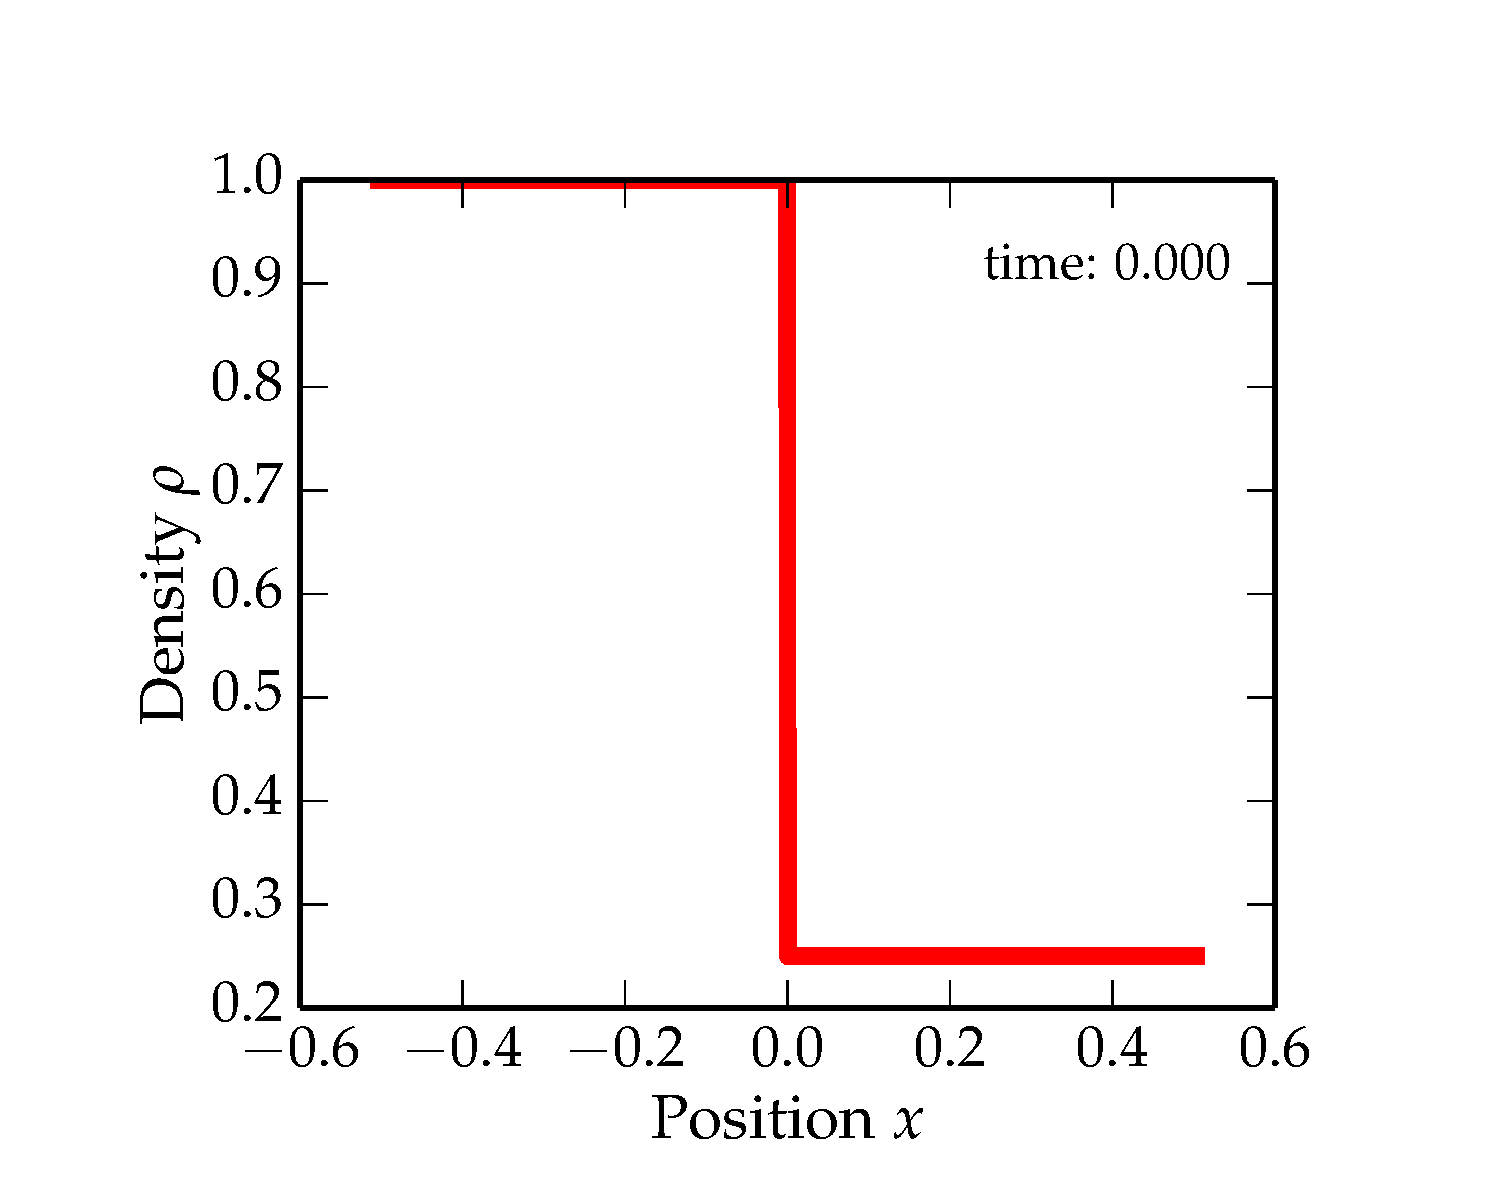
\includegraphics[width=0.75\textwidth]{figs-pc/0.pdf}
 \caption{Initial density profile.}
\end{figure} 

\begin{figure}[H]
 \centering
 \hspace{0cm} 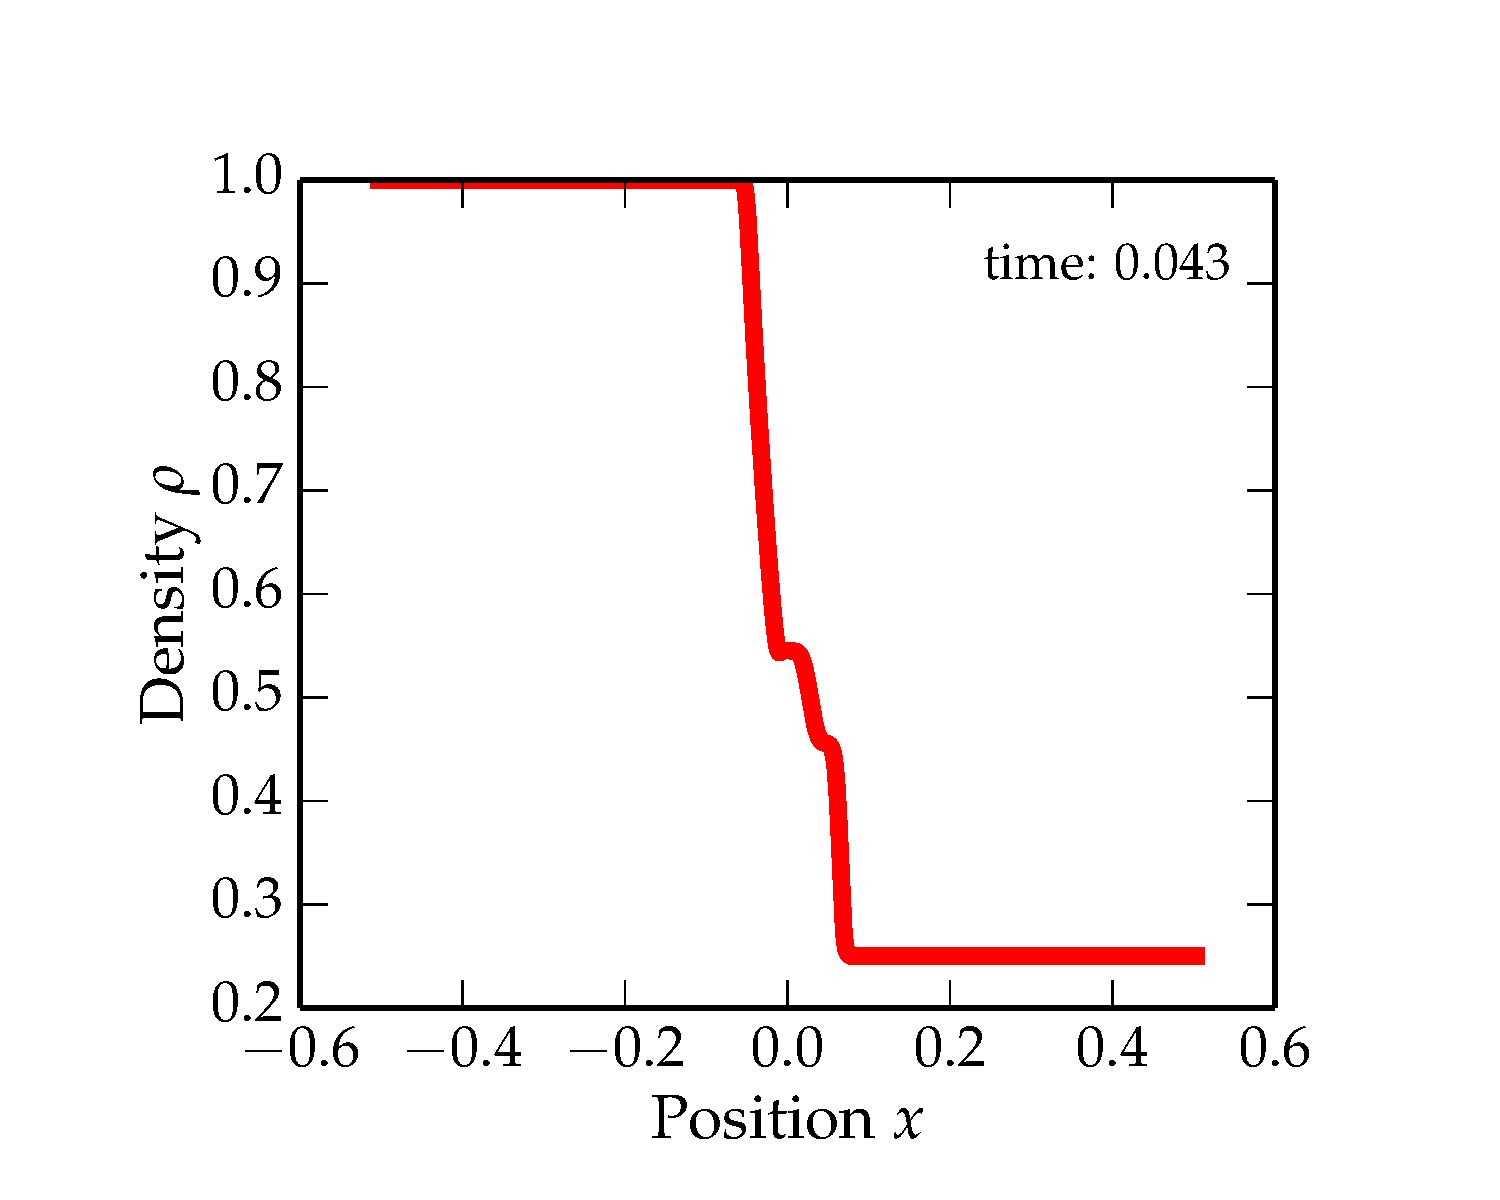
\includegraphics[width=0.75\textwidth]{figs-pc/200.pdf}
 \caption{Density profile at the 200th simulation iteration, which corresponds to a time of 0.043.}
\end{figure} 

\begin{figure}[H]
 \centering
 \hspace{0cm} 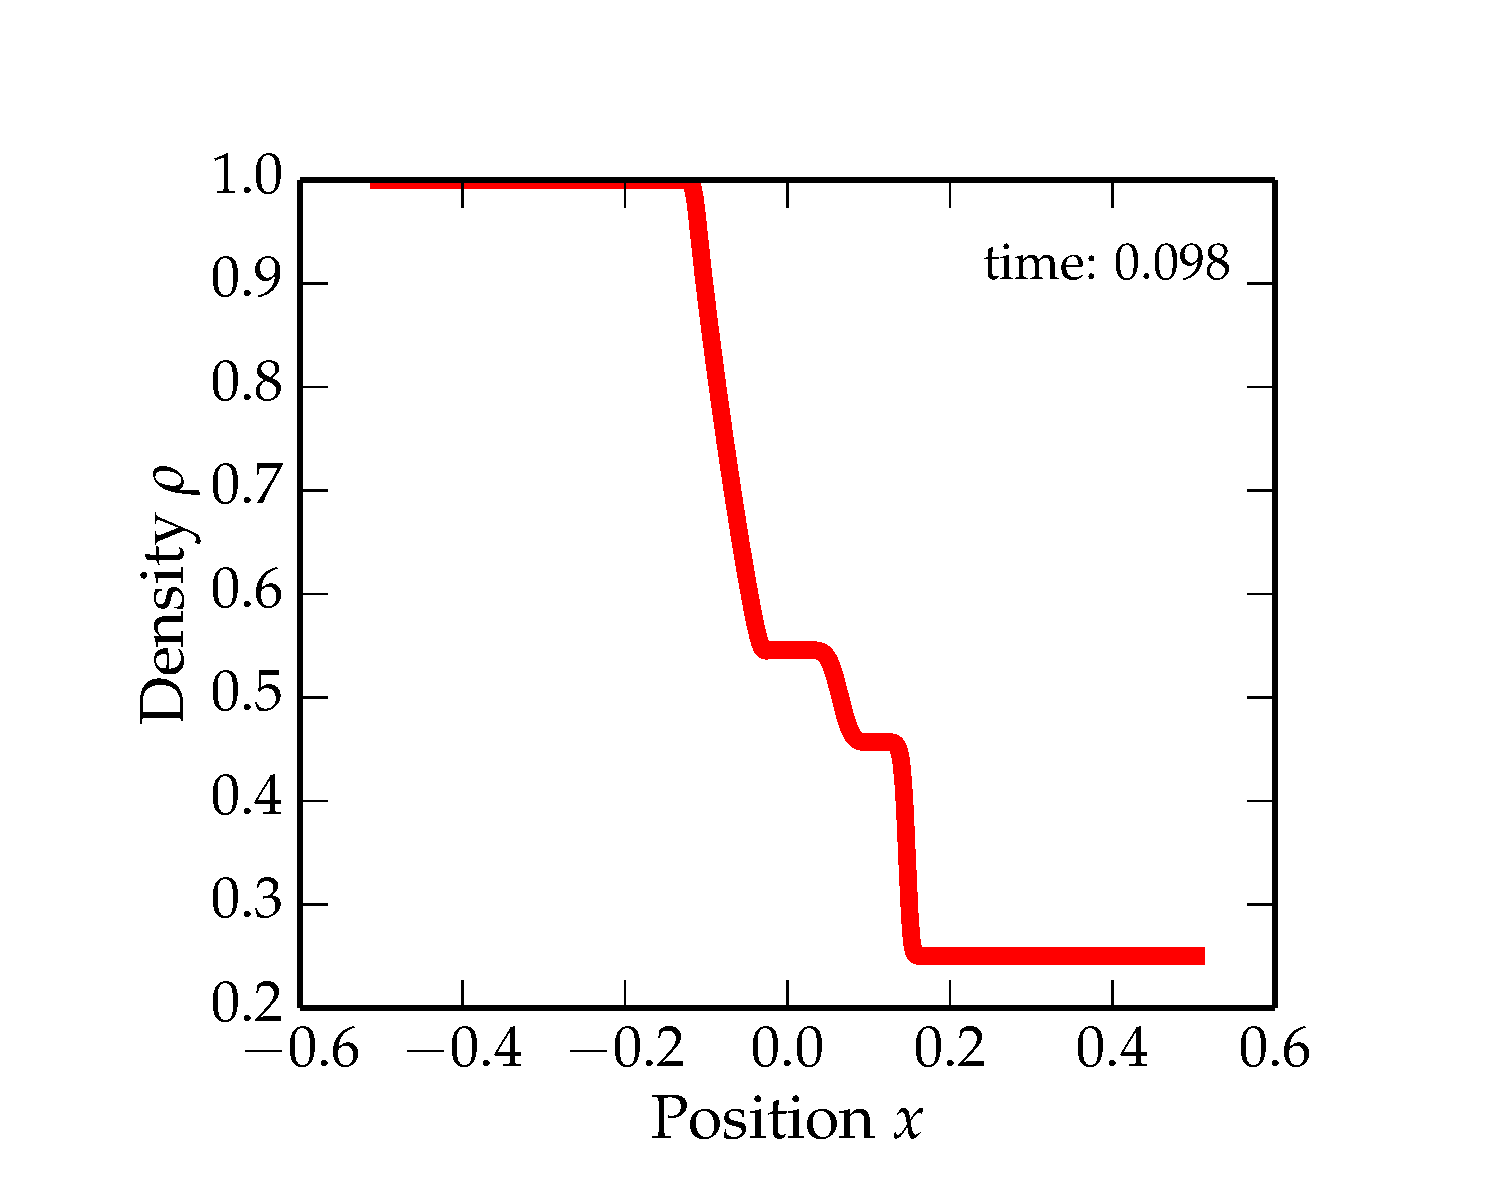
\includegraphics[width=0.75\textwidth]{figs-pc/400.pdf}
 \caption{Density profile at the 400th simulation iteration, which corresponds to a time of 0.098.}
\end{figure} 

\begin{figure}[H]
 \centering
 \hspace{0cm} 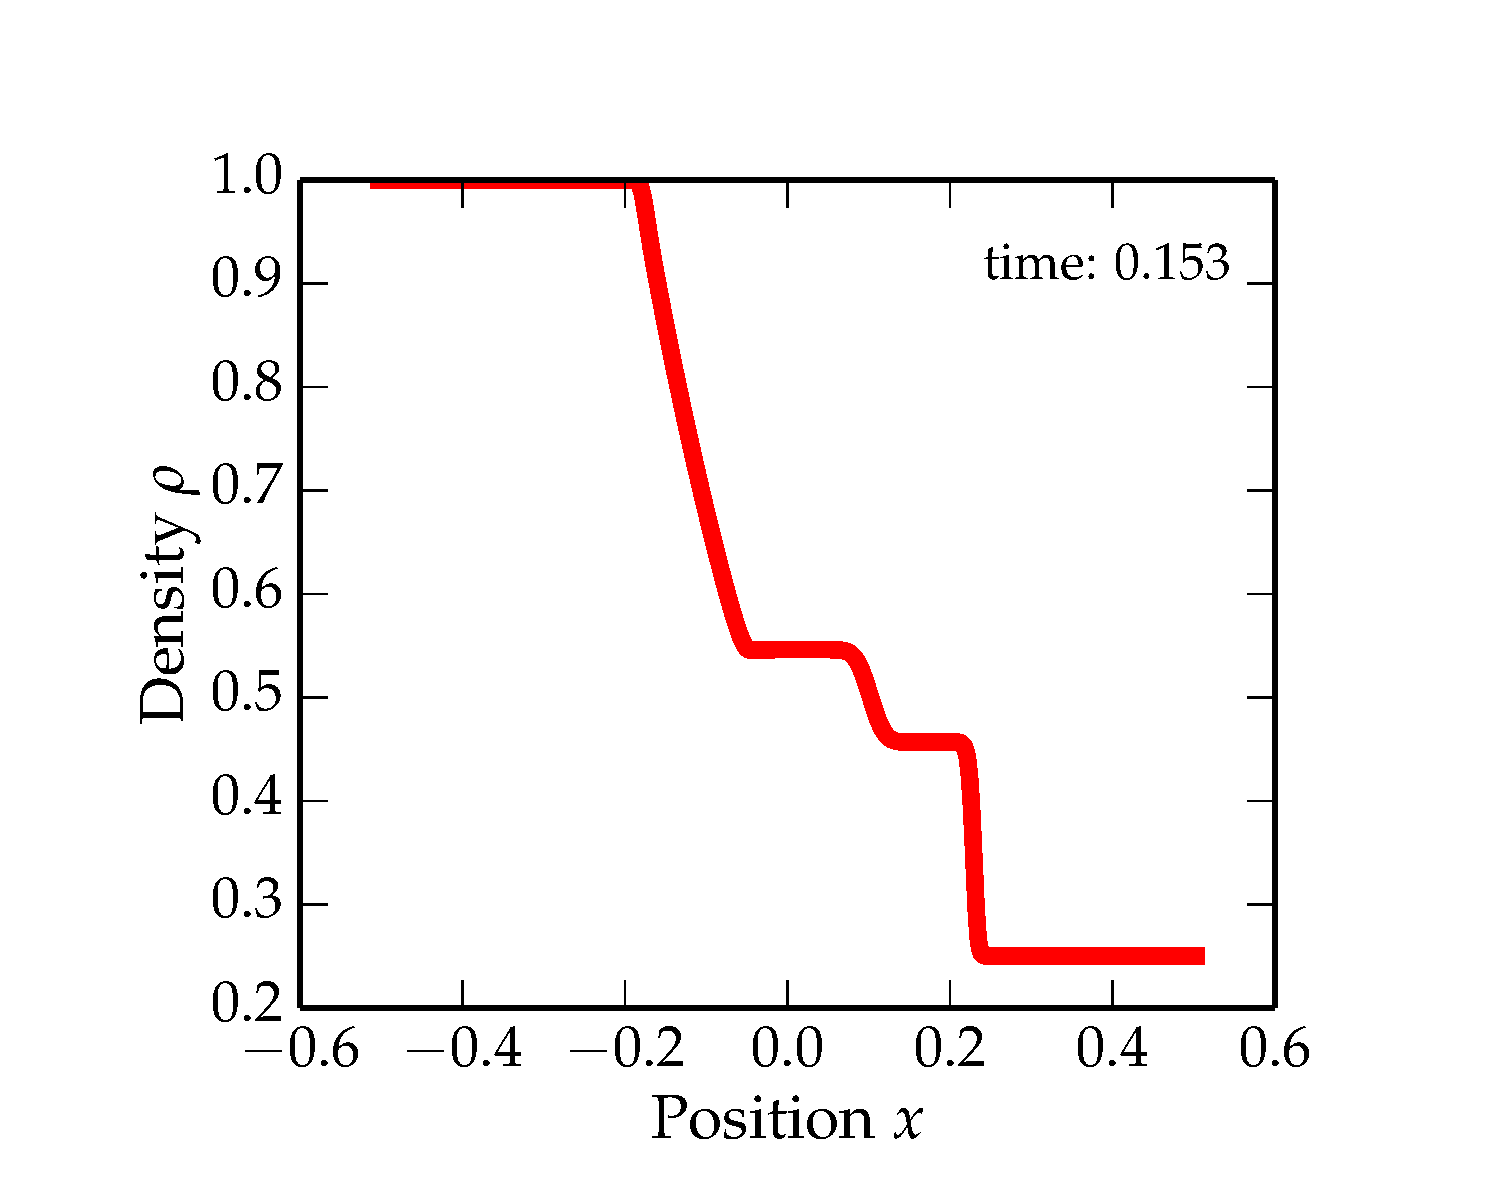
\includegraphics[width=0.75\textwidth]{figs-pc/600.pdf}
 \caption{Density profile at the 600th simulation iteration, which corresponds to a time of 0.153.}
\end{figure} 

\begin{figure}[H]
 \centering
 \hspace{0cm} 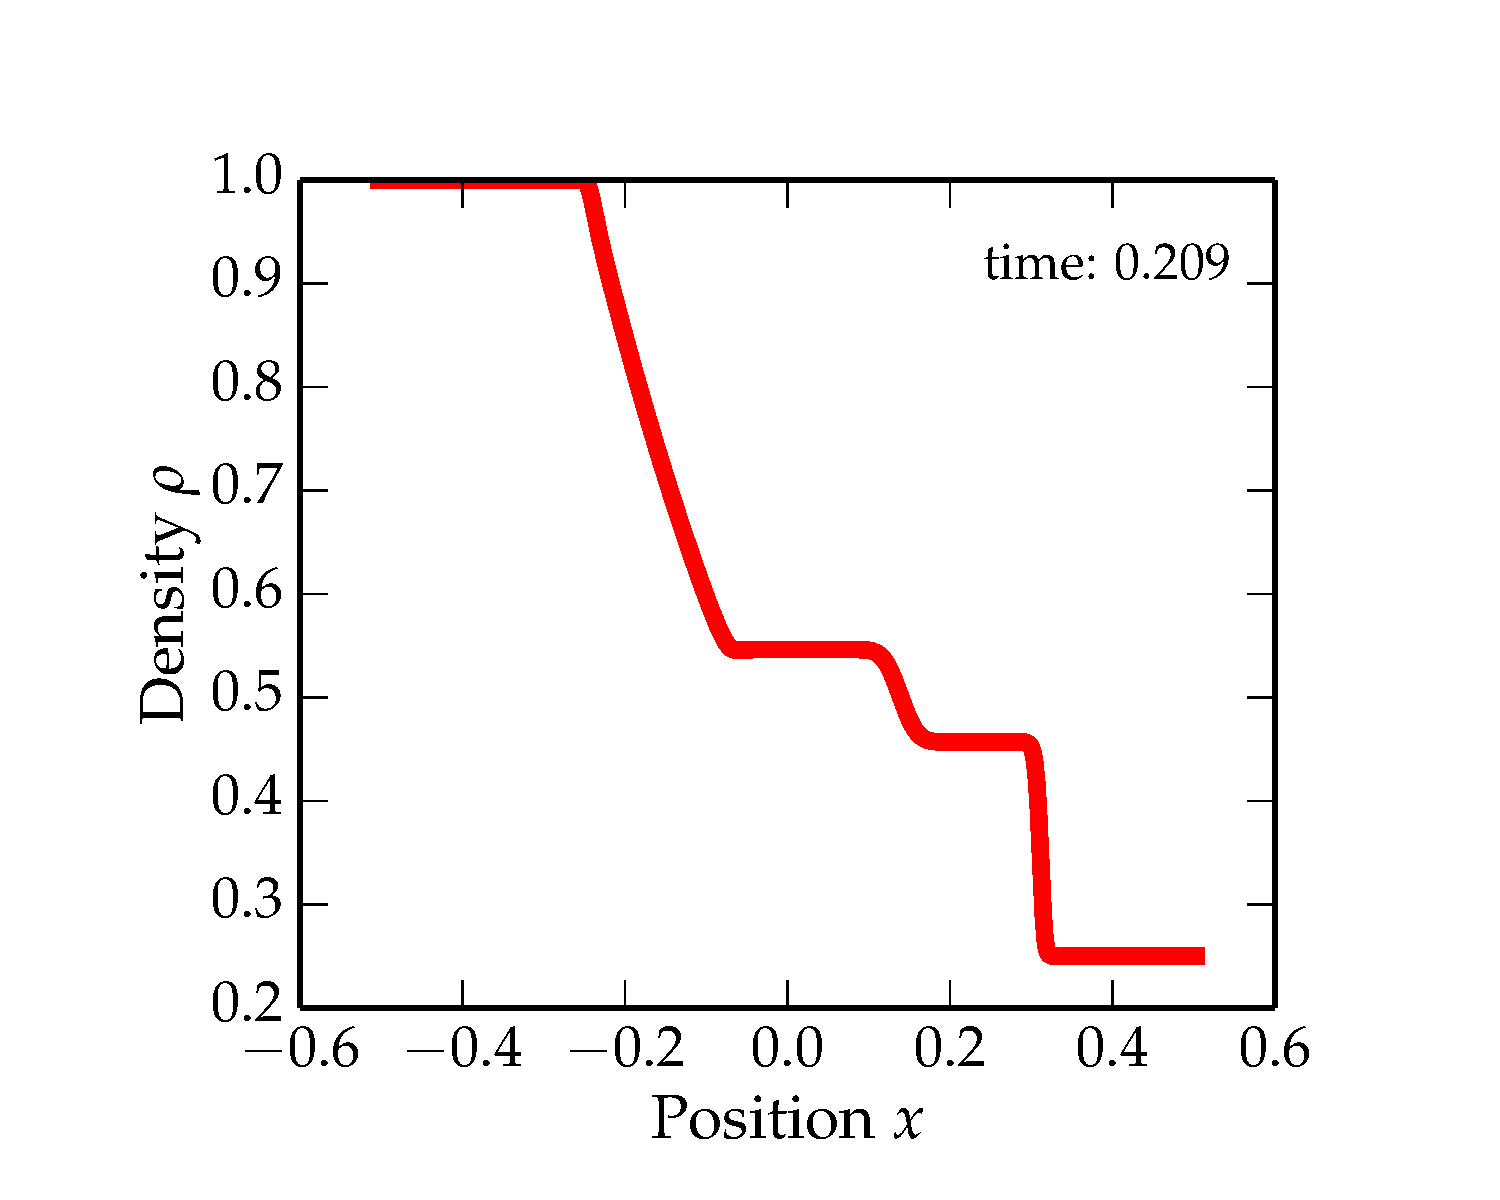
\includegraphics[width=0.75\textwidth]{figs-pc/800.pdf}
 \caption{Density profile at the 800th simulation iteration, which corresponds to a time of 0.209.}
\end{figure} 

\newpage
\noindent \textbf{2.}

I then compared the simulation results at time \(t = 0.2\) for the piecewise-constant, TVD-minmod, and TVD-MC2 reconstruction methods, as shown in Figure~6.

\begin{figure}[H]
 \centering
 \hspace{0cm} 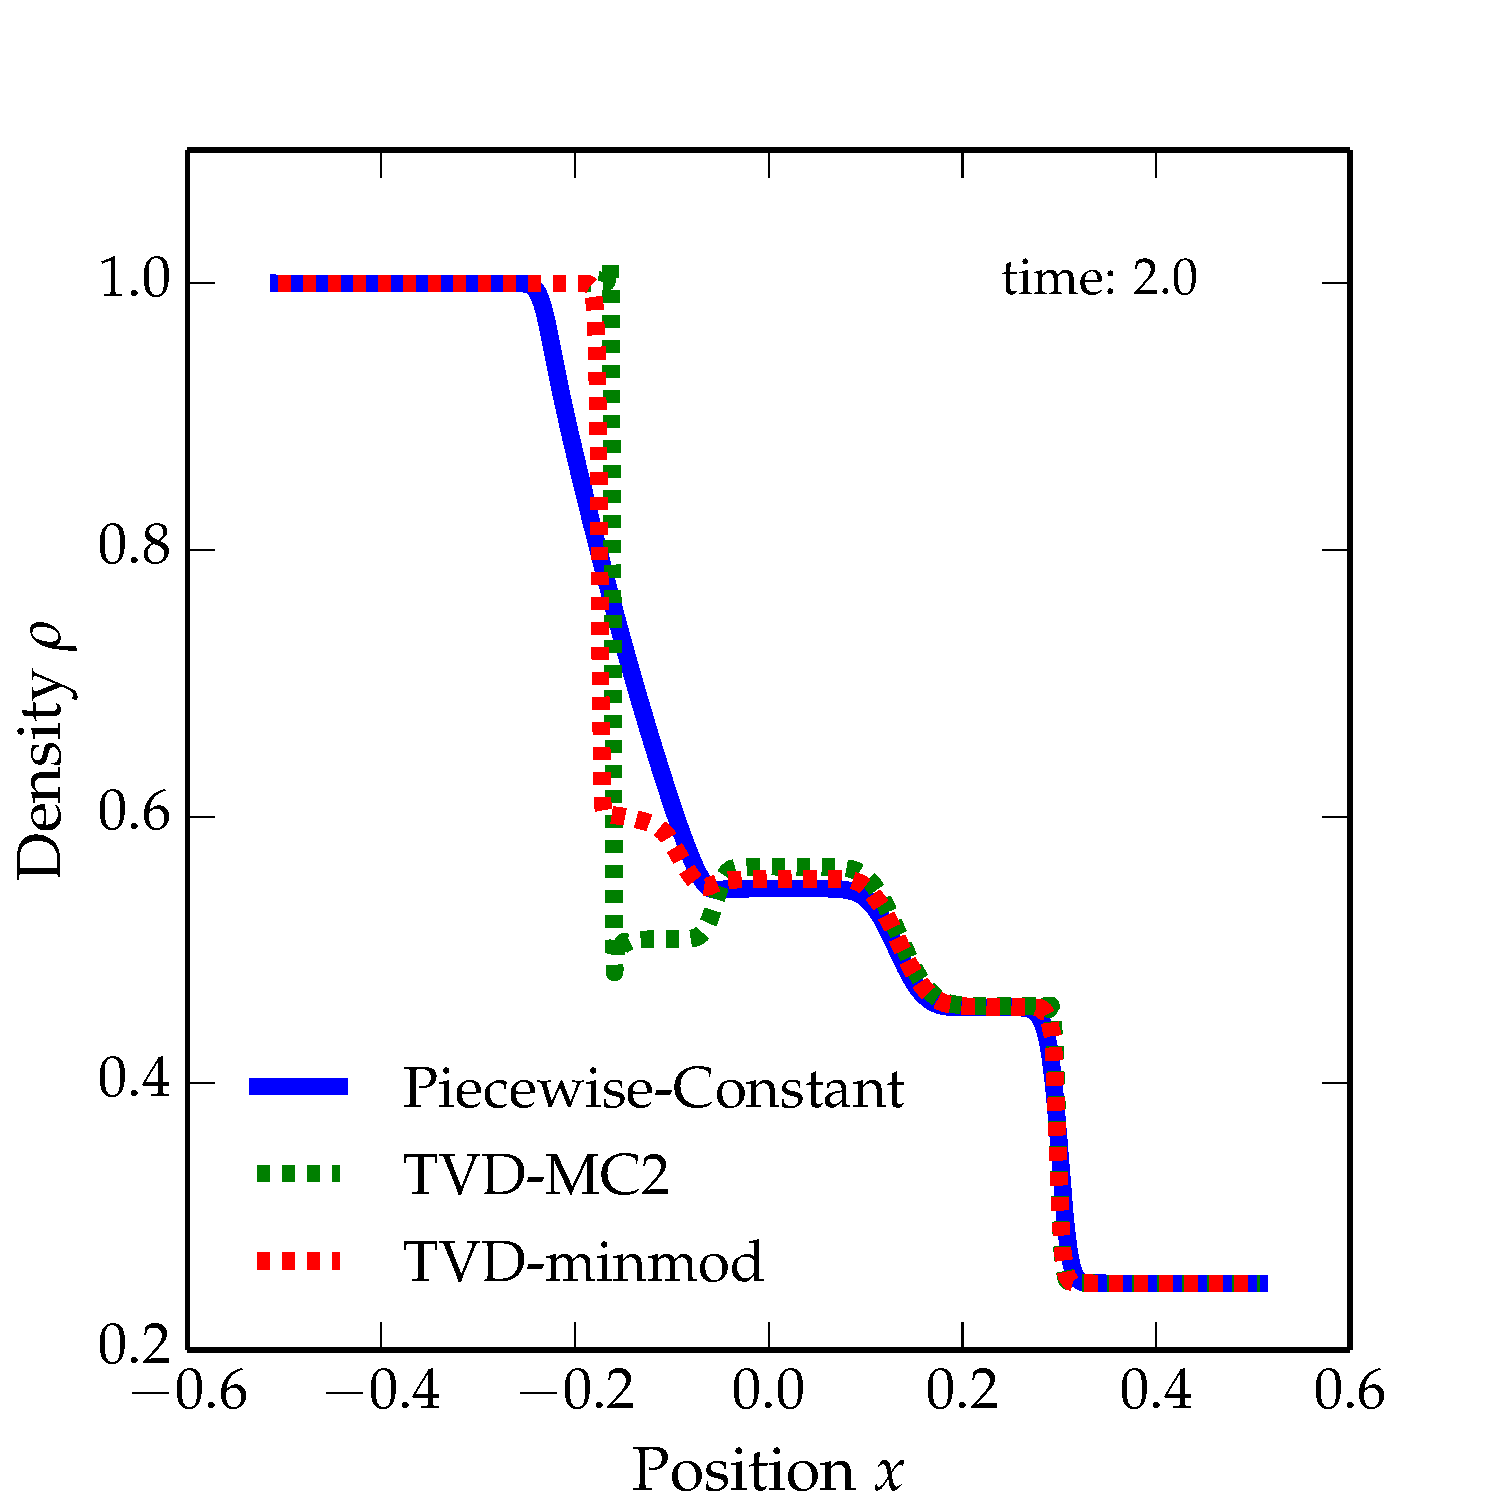
\includegraphics[width=0.75\textwidth]{comparison.pdf}
 \caption{Density profile at time \(t = 0.2\) for simulations run with the piecewise-constant, TVD-MC2, and TVD-minmod reconstruction methods. It is clear that the two TVD methods produce more features in the density profile, such as the rarefaction layer.}
\end{figure}

\noindent \textbf{3.}

I then compared the results of this 1D finite volume hydro code with the results of the 1D smooth particle hydrodynamics code from WS15 set up with the same initial conditions. The reconstruction method for the finite volume hydro code that produces a density profile closest to the analytic result is TVD-minmod, as can be seen from Figure~6. I compare the TVD-minmod result (Figure~7) to the SPH result (Figure~8) at \(t = 0.2\) below. These produce extremely disparate results; while the finite volume hydro code decreases in density monotonically moving from left to right, the SPH code results in a large local maximum in density at the location where the shock discontinuity is in the finite volume code. 

I couldn't get my Fortran compiler to work, so I'm skipping that part.\\

\noindent \textbf{4.}

I sped up my code by using \texttt{numpy} array operations instead of slow loops; the result is in \texttt{ws16\_sped-up.py}. The run-time of the old code is \(216.5 \pm 4.0\) seconds, whereas the run-time of the new code is \(163.0 \pm 1.5\) seconds, a speed-up of 25\%.

\begin{figure}[H]
 \centering
 \hspace{0cm} 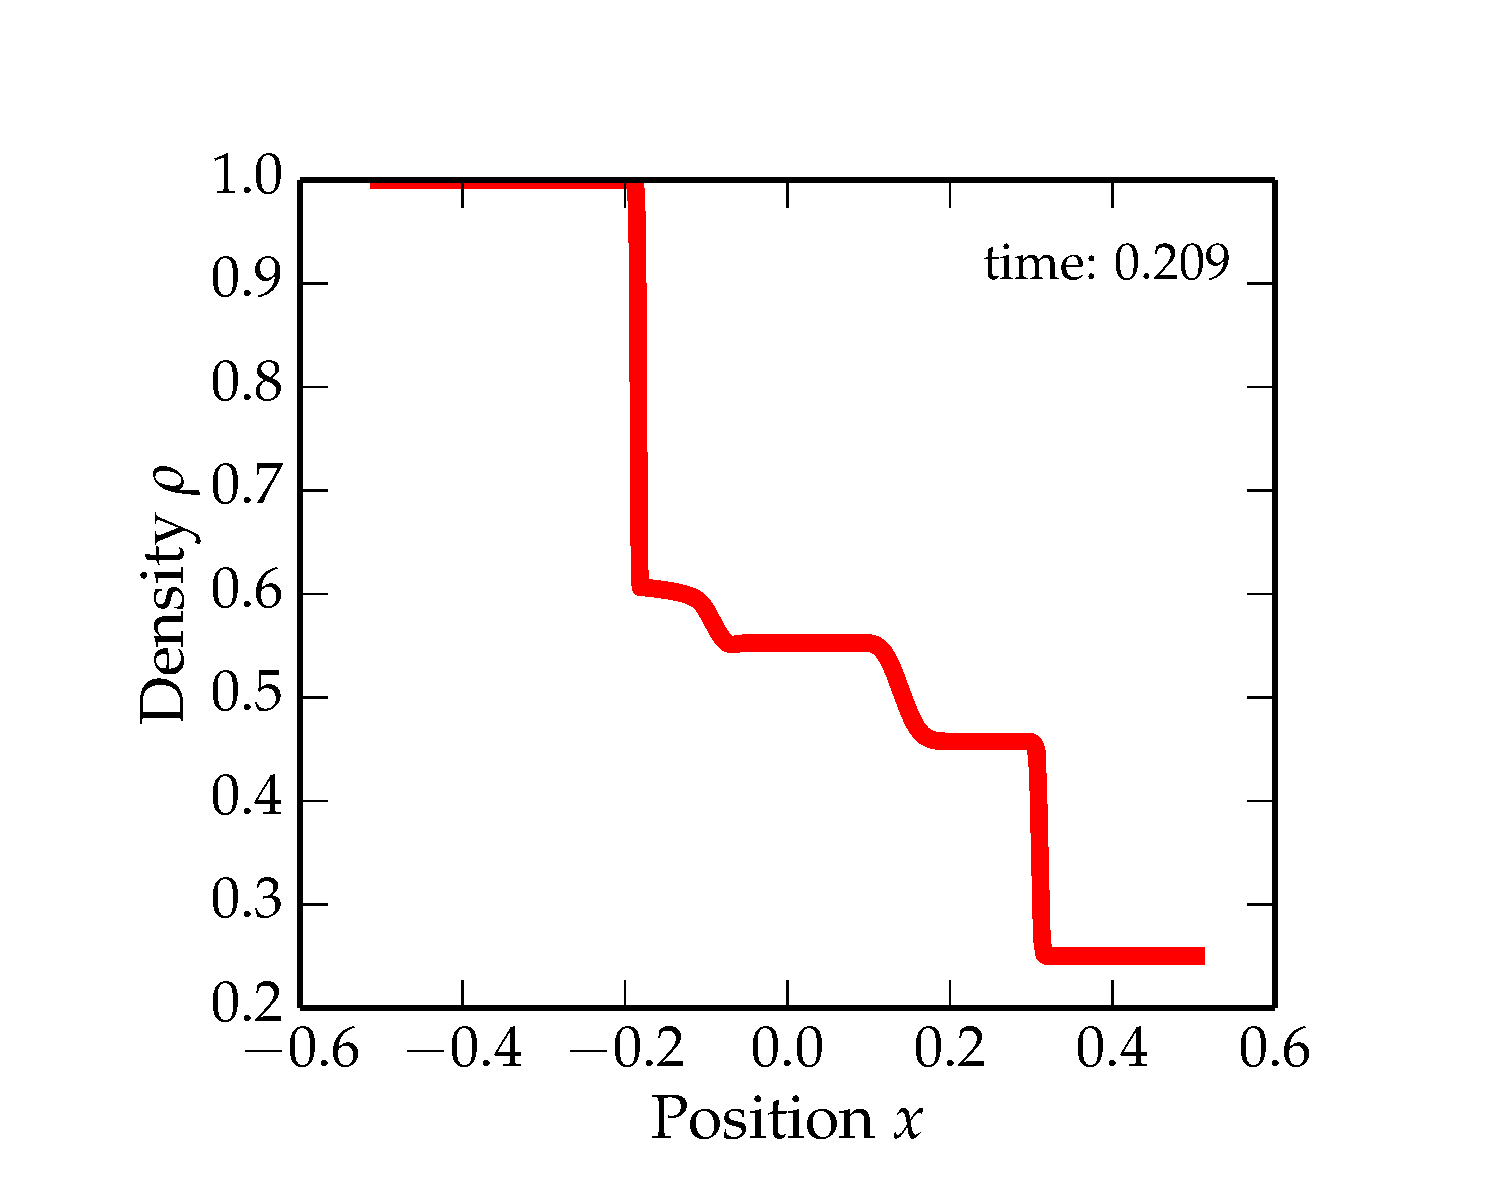
\includegraphics[width=0.75\textwidth]{minmod.pdf}
 \caption{Density profile at time \(t = 0.2\) for the finite volume hydro code with TVD-minmod reconstruction.}
\end{figure}

\begin{figure}[H]
 \centering
 \hspace{0cm} \includegraphics[width=0.75\textwidth]{sph.pdf}
 \caption{Density profile at time \(t = 0.2\) for the SPH code.}
\end{figure}



\end{spacing}
\end{document}

%%%%%%%%%%%%%%%%%%%%%%%%%%%%%%%%%%%%%%%%%%%%%%%%%%%%%%%%%%%%%
